\chapter{Propriétés génériques d'un capteur}
\section{Capteur idéal (erreur nulle)}
\subsection{Loi du capteur}
Notons:
\begin{description}
	\item[X] la grandeur physique à mesurer (entrée du transducteur).
	\item[S] la grandeur électrique après conversion (sortie du transducteur).
\end{description}
Ainsi, la loi \(S=\text{fct}(X)\) est appelée \emph{caractéristique}. En supposant cette caractéristique connue, nous pouvons retrouver l'entrée \(X\) à partir de la valeur de sortie du transducteur.
\begin{figure}[H] 
	\centering 
	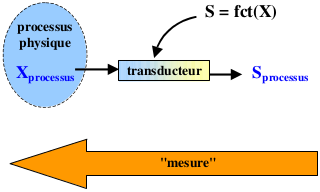
\includegraphics[width=0.4\textwidth]{ch2/image1} 
	\caption{Principe d'une mesure: cas idéal}
\end{figure} 
Cette caractéristique s'appelle plus exactement la \emph{loi du capteur}. Elle peut se représenter schématiquement ou mathématiquement. 
\begin{figure}[H] 
	\centering 
	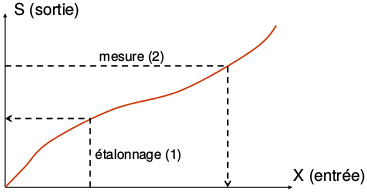
\includegraphics[width=.5\textwidth]{ch2/image2} 
	\caption{Loi du capteur}
\end{figure}
Remarquons que même si l'on dispose de l'expression mathématique, on obtient cette loi toujours sur base d'un \emph{étalonnage} (ou calibration) en imposant des valeurs d'entrée (connues) et relevant les valeurs de sortie correspondantes. Il y a néanmoins une subtilité, l'étalonnage ne peut s'effectuer qu'avec des \emph{valeurs de référence} stables et connues.\\

De l'étalonnage découle 2 propriétés fondamentales:
\begin{description}
	\item[gamme de mesure] la gamme de valeurs de \(X\) acceptée par le capteur, c-à-d la gamme pour laquelle le capteur fonctionne avec une erreur < erreur de précision nominale. Cette gamme se trouve sur chaque datasheet.
	\item[sensibilité] rapport entre la variation de \(S\) et la variation correspondante de \(X\), c-à-d \(s(X)=\left.\frac{\Delta S}{\Delta X}\right|_X\), la pente de la loi du capteur. De manière générale, \(s\) varie en fonction de \(X\). Si \(s=cste\), alors le capteur est \emph{linéaire} (une variation de \(X\) à différents endroits de l'étendue de mesure donne la même variation de \(S\) en amplitude).
\end{description}
On en conclu donc qu'il est préférable d'avoir une sensibilité \emph{élevée} et \emph{constante}.
\begin{figure}[H] 
	\centering 
	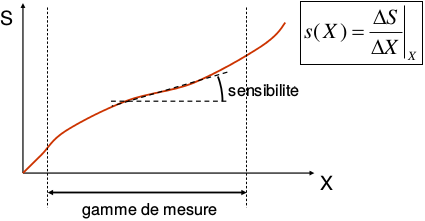
\includegraphics[width=0.5\textwidth]{ch2/image3} 
	\caption{Loi du capteur: propriétés}
\end{figure}
\section{Capteur réel (erreur non nulle)}
\subsection{Principe d'une mesure: erreurs et précision}
\begin{figure}[H] 
	\centering 
	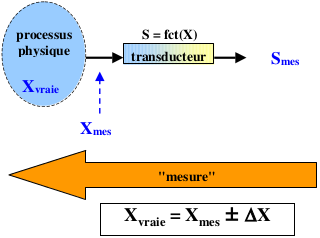
\includegraphics[width=0.4\textwidth]{ch2/image4}
	\caption{Principe de mesure: cas réel} 
\end{figure}
Évidement, dans le cas réel, la grandeur \(X\) déduite de la mesure est \(\neq\) valeur exacte de \(X\) (dû à plein de raisons que l'on verra plus tard). On distingue donc 3 valeurs:
\begin{description}
	\item[valeur vraie (\(X_{\text{vraie}}\))] valeur exacte de la grandeur à mesurer. Grandeur que l'on aimerait connaître mais qui en pratique est inaccessible car se trouvant avant le capteur (non idéal).
	\item[valeur mesurée à la sortie du capteur (\(S_{\text{mes}}\))] valeur de la grandeur \(S\) délivrée en pratique par le capteur.
	\item[valeur mesurée à l'entrée du capteur (\(X_{\text{mes}}\))] la traduction de \(S_{\text{mes}}\) connaissant la loi du capteur.
\end{description} 
\(X_{\text{mes}}\) n'est autre qu'une \emph{approximation} de \(X_{\text{vraie}}\). Il devient donc important de connaître la qualité de l'approximation.\\

La qualité de l'approximation est définie par:
\begin{description}
	\item[précision (du capteur)] aptitude à donner une valeur mesurée proche de la valeur vraie (notion qualitative).
	\item[erreur de précision \(\Delta X\)] écart maximal entre la valeur vraie et la valeur mesurée (notion quantitative). Ceci est communément appelée « erreur ».
\end{description}
\subsection{Sources d'erreurs}
Les causes des différences entre \(X_{\text{vraie}}\) et \(X_{\text{mes}}\) sont des erreurs classées selon 3 types:
\begin{itemize}
	\item les erreurs accidentelles (ou conditionnelles)
	\item les erreurs stochastiques
	\item les erreurs systématique
\end{itemize}
On distingue 2 propriétés:
\begin{description}
	\item[fidélité (ou répétabilité)] aptitude à donner des valeurs mesurées concordantes entre elles pour une même valeur de la valeur vraie, c-à-d ayant une faible dispersion des mesures (notion qualitative). Elle est caractérisée quantitativement par l'\emph{erreur de fidélité}. 
	\item[justesse] aptitude à donner une valeur mesurée proche de la valeur vraie (notion qualitative). Elle est caractérisée quantitativement par l'\emph{erreur de justesse}.
\end{description}
On en déduit donc que la justesse est liée aux erreurs systématiques (un système dont l'erreur systématique est faible est "juste") alors que la fidélité est liée aux erreurs accidentelles (un système a faible erreur accidentelles est "fidèle").

L'erreur de précision est donc la \(\sum\) erreurs de justesse et fidélité.
\begin{figure}[H]
	\centering 
	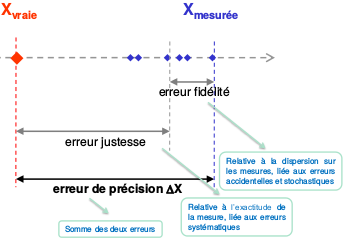
\includegraphics[width=.5\textwidth]{ch2/image5}
	\caption{Précision, fidélité et justesse}
\end{figure}
\subsubsection{Erreurs accidentelles (ou conditionnelles)}
L'erreur accidentelle est d'origine extérieure, pouvant être variable d'une mesure à l'autre. Les exemples typiques sont des erreurs de lecture (maison construite en cm et pas en m) et des parasites (\danger pas du bruit, le bruit est interne, les parasites externes).
\subsubsection{Erreurs stochastiques}
L'erreur stochastique est d'origine interne, pouvant être variable d'une mesure à l'autre \(\Rightarrow\) Bruit. Contrairement aux erreurs accidentelles, le bruit peut être prédit.
\subsubsection{Erreurs systématiques}
Il y a tous d'abord des erreurs dues à des distorsions par rapport à la caractéristique supposée du capteur. Il y a deux types de distorsions:
\begin{description}
	\item[linéarité] erreur de linéarité est le plus grand écart entre la courbe d'étalonnage réelle et la meilleure droite obtenue par régression.
	\item[réversibilité \textnormal{ou} hystérèse] la réversibilité est l'aptitude à fournir une même valeur de sortie pour une valeur d'entrée obtenue successivement par variation croissante et décroissante. Ainsi, la différence entre ces 2 valeurs est l'erreur d'hystérésis.
\end{description}
Ces erreurs peuvent provenir soit d'une connaissance imparfaite du capteur (caractéristique différente de celle prévue initialement), soit de l'utilisation (consciente) d'un modèle simplifié de la loi du capteur (en utilisant par exemple une loi linéaire alors qu'elle ne l'est rigoureusement pas).
\begin{figure}[H]
	\centering 
	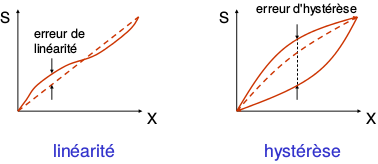
\includegraphics[width=0.7\textwidth,height=10\baselineskip,keepaspectratio]{ch2/image6}
	\caption{Erreurs de linéarité et hystérèse}
\end{figure}

Ensuite, il y a les erreurs dues à la résolution (milieu numérique), définie comme la plus petite variation de la grandeur d'entrée qui provoque coup sûr une variation de la grandeur de sortie.
\begin{figure}[H] 
	\centering 
	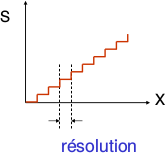
\includegraphics[width=0.6\textwidth,height=8\baselineskip,keepaspectratio]{ch2/image7}
	\caption{Erreur de résolution}
\end{figure}
Enfin, il y a les erreurs dues aux grandeurs d'influence, c-à-d que la grandeur de sortie S ne va pas varier qu'en fonction de X, mais aussi d'une grandeur physique Z "parasite" (:= grandeur d'influence) comme la température (plus courante), pression, etc. On distingue 2 types d'erreur:
\begin{itemize}
	\item accidentelle : la sortie varie d'une mesure à l'autre à cause des grandeurs d'influence (genre température)
	\item systématique : la caractéristique varie lentement en fonction d'une grandeur d'influence (genre vieillissement\footnote{Ou aussi la température, dans le cas par exemple d'un transistor dont les propriétés sont différentes "à chaud" et "à froid"}). On parle de \emph{dérive} du capteur
\end{itemize}
\begin{figure}[H] 
	\centering 
	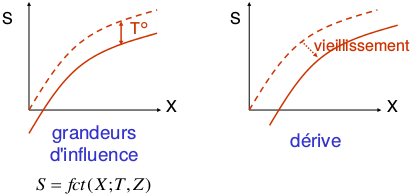
\includegraphics[width=0.7\textwidth,height=10\baselineskip,keepaspectratio]{ch2/image8}
	\caption{Grandeurs d'influence et dérive}
\end{figure}
\subsubsection{Domaines d'utilisation}
Il peut arriver que l'entrée sorte de la gamme prévue, pouvant modifier le fonctionnement du capteur. On distingue:
\begin{itemize}
	\item Le domaine nominal d'utilisation: grandeur d'entrée X et grandeurs d'influence peuvent s'y trouver de manière permanente sans altérer la précision du capteur
	\item Le domaine de non détérioration: propriétés du capteur altérées (par exemple erreur > erreur nominale), mais de manière réversible \(\rightarrow\) le capteur retrouve ses propriétés nominales lorsqu'on retourne dans le domaine nominal 
	\item Le domaine de non destruction: propriétés altérées de manière irréversible mais le capteur continue de fonctionner 
	\item Le domaine de destruction: le capteur ne fonctionne plus
\end{itemize}
Contrairement à ce qu'on pourrait penser, on utilise parfois le capteur hors de son domaine nominal. Par exemple, la précision d'un thermocouple (capteur de température) n'est garantie que pour sa première mesure car il vieillit vite, l'utiliser plus d'une fois (quand une grande précision n'est pas requise) revient à l'utiliser hors de son domaine nominal.

\section{Propriétés dynamiques}
Précédemment, les propriétés étaient \emph{statiques}, c-à-d avec l'hypothèse que \emph{les grandeur(s) d'entrée(s) variai(en)t lentement (voir pas du tout) par rapport au temps de réaction du système de mesure}. Les propriétés dynamiques sont les propriétés qui:
\begin{itemize}
	\item ne satisfont pas l'hypothèse précédente
	\item portent sur toute variation des grandeurs statiques en fonction de la fréquence
	\item ont besoin de caractériser la vitesse de réponse du capteur/système
\end{itemize}
\subsection{Principales propriétés}
On distingue plusieurs propriétés:
\begin{description}
	\item Réponse en fréquence \(s(f)\)
	\begin{itemize}
		\item variation de la sensibilité en fonction de la fréquence
		\item réponse en fréquence = amplitude + phase
		\item limite BF et HF
	\end{itemize}
	\item Bande passante
	\begin{itemize}
		\item gamme de fréquence d'utilisation du capteur
		\item définie par un affaiblissement de \(\SI{3}{\decibel}\) de la réponse en fréquence
	\end{itemize}
	\item Réponse indicielle \(S(t)\)
	\begin{itemize}
		\item réponse temporelle à un échelon sur la grandeur d'entrée
		\item liée à la réponse en fréquence
	\end{itemize}
	\item Ordre du système
	\begin{itemize}
		\item ordre de la dérivée la plus élevée dans l'équation différentielle du système
		\item grande majorité des capteurs \(\rightarrow\) 1\up{er} ou 2\up{ème} ordre
	\end{itemize}
\end{description}
\subsection{Système du premier ordre (ex. circuit RC)}
Équation différentielle du 1\up{er} ordre:
\[
a\frac{d S(t)}{dt} + b S(t) = X(t)\qquad a, b=\cst
\]
La réponse en fréquence (avec \(f_0\) = fréquence de coupure):
\[
|s(f)|=\frac{s(0)}{\sqrt{1+\left(\frac{f}{f_0}\right)^2}}\qquad \arg[s(f)] = -\arctan\left(\frac{f}{f_0}\right)\qquad f_0=\frac{b}{2\pi a}
\]
La réponse indicielle (\(\tau\) = cst de temps):
\[
S(t) = \frac{X_0}{b}\left(1-e^{-t/\tau}\right)\qquad \tau =\frac{a}{b}=\frac{1}{2\pi f_0}
\]
\begin{figure}[H] 
	\centering 
	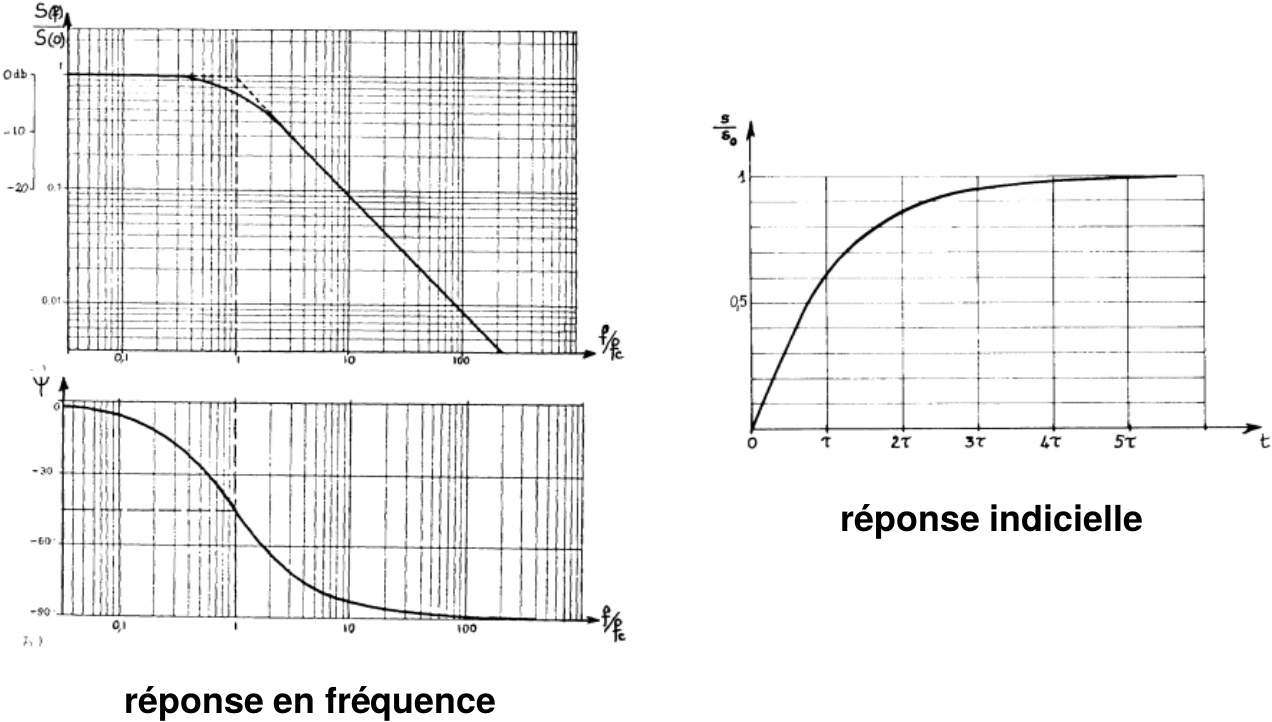
\includegraphics[width=0.7\textwidth]{ch2/image10} 
	\caption{Système du 1\up{er} ordre} 
\end{figure}
\subsection{Système du second ordre (ex. circuit RLC)}
Équation différentielle du 2\up{ème} ordre:
\[
a\frac{d^2 S(t)}{dt^2} + b \frac{d S(t)}{dt} + cS(t) = X(t)\qquad a,b,c=\cst
\]
En définissant \(f_0\) = fréquence propre et \(\zeta\) = coefficient d'amortissement
\[
f_0 = \frac{1}{2\pi}\sqrt{\frac{c}{a}}\qquad \zeta=\frac{b}{2\sqrt{c\,a}}
\]
nous obtenons la réponse en fréquence:
\[
|s(f)|=\frac{s(0)}{\sqrt{1-\left(\frac{f}{f_0}\right)^2+4\zeta^2\left(\frac{f}{f_0}\right)^2}}\qquad \arg[s(f)] = -\arctan\left(\frac{2\zeta}{\frac{f_0}{f}\left[1-\left(\frac{f}{f_0}\right)^2\right]}\right)
\]

\begin{figure}[H] 
	\centering 
	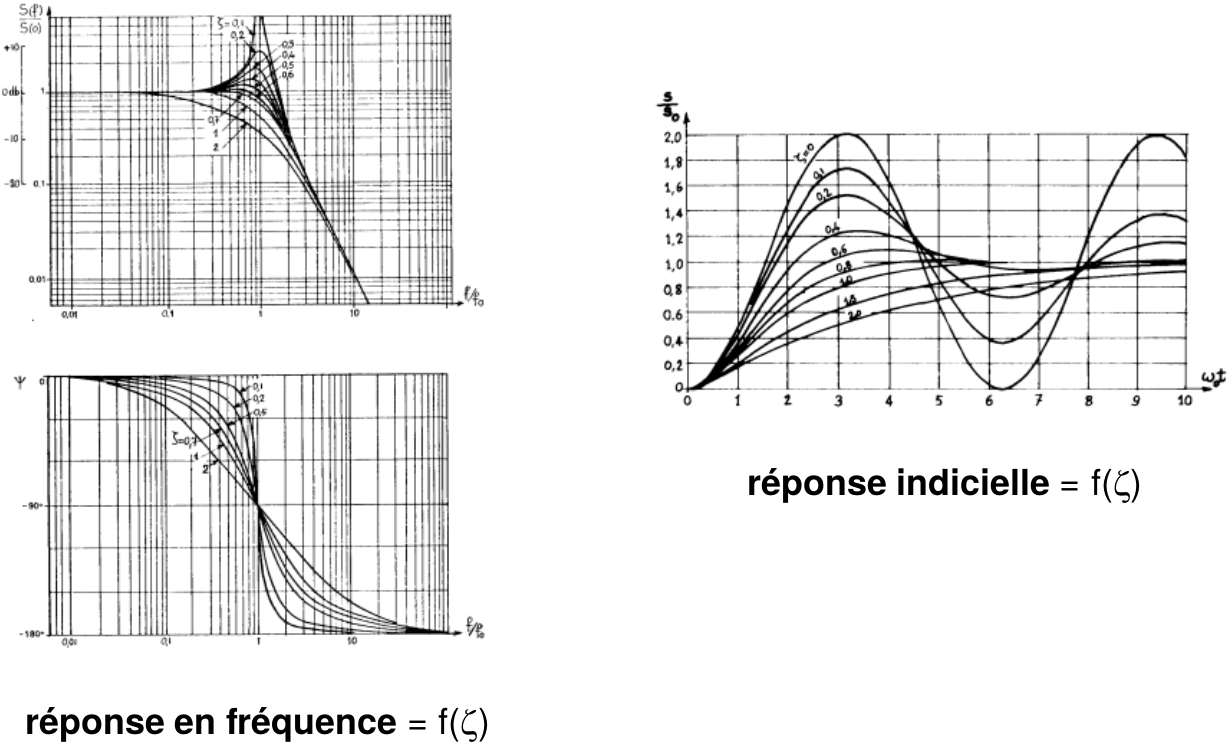
\includegraphics[width=0.8\textwidth]{ch2/image11} 
	\caption{Système du 2\up{ème} ordre} 
\end{figure}
\subsection{Temps de réponse}
Le temps de réponse (ou temps d'établissement) est la \emph{durée minimale d'attente, après application d'un échelon à l'entrée, pour que l'écart relatif de la sortie par rapport à sa valeur finale demeure constamment inférieur à \(\epsilon\)\%}
\begin{figure}[H] 
	\centering 
	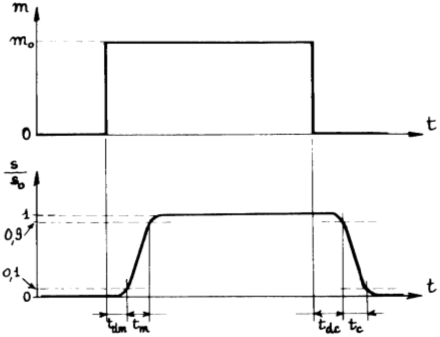
\includegraphics[width=0.8\textwidth,height=10\baselineskip,keepaspectratio]{ch2/image12} 
	\caption{Temps d'établissement} 
	\label{fig:tempsétabliss}
\end{figure}
\paragraph{Remarque:} le temps de réponse \(\neq\) temps de montée car cela comprend aussi les éventuels retards de la chaîne ou du capteur. De plus, nous n'arrivons jamais à 1 (\autoref{fig:tempsétabliss}) car \(1-e^{-t/\tau}\neq 1\), on prend donc une caractéristique entre 10 et 90\%.
\section{Autres propriétés}
Avant de décrire cette section, rajoutons qu'en plus des propriétés décrites ci-dessous, il existe les propriétés de coût, de dimensions et d'encombrement, d'ambiance supportée (parasite, atmosphère corrosive).
\subsection{Transducteur actif >< passif}
On distingue 2 type de transducteur:
\begin{description}
	\item[actif] peut être assimilé à une source (sens électrique, courant, tension, charge) dont la valeur varie en fonction de la grandeur à mesurer (énergie vient du processus).
	\item[passif] peut être assimilé à un composant passif (impédance variable) dont la valeur varie en fonction de la grandeur mesurée (énergie vien de la chaîne d'acquisition).
\end{description}
\subsection{Reproductibilité et finesse}
\begin{description}
	\item[Finesse] aptitude d'un capteur à ne pas modifier (par sa présence) la grandeur mesurée. La finesse est exprimée par la valeur d'une grandeur physique déterminant l'inertie du capteur par rapport au mesurande (ex. capacité calorifique d'un capteur thermique ou moment d'inertie d'un potentiomètre mécanique). Varie dans le même sens que la rapidité mais inversement par rapport à la sensibilité.
	\item[Reproductibilité (>< fidélité)] aptitude à obtenir une même valeur de la grandeur de sortie lorsque la mesure est effectuée au moyen de différents instruments, par différents opérateurs, en des lieux et temps différents.
\end{description}
\subsection{fiabilité/maintenance}
\begin{description}
	\item["Reliabilité"] probabilité qu'a le système de fonctionner correctement (propriétés non affectées) après une période de temps définie.
	\item[MTBF (mean time between failure)] durée moyenne de bon fonctionnement entre deux pannes successives.
	\item[Maintenabilité] aptitude du capteur à être disponible le plus longtemps possible, c-à-d à donner des informations permettant une maintenance préventive (but: remplacer avant la panne).
	\item[Interchangeabilité] aptitude du capteur à se substituer à un autre capteur dans altérer les performances de la chaîne de mesure.
	\item[Interopérabilité] aptitude de différents capteurs et instruments de mesure à être utilisés ensemble et à échanger des données (capteurs intelligents).
\end{description}
\subsection{fonctions de haut niveau}
Les fonctions de haut niveau ont pour but de centraliser la chaîne d'acquisition en 1 endroit. Ceci est plus intelligent car il ne faut plus transmettre toutes les informations et la batterie est moins sollicitée.
\begin{description}
	\item[capteur intégré] conditionneur intégré sur le même silicium que le capteur
	\item[capteur à la sortie numérique] conversion A/N intégrée au capteur avec différentes interfaces de sorties possibles
	\item[capteur intelligent] capacité de traitement (microcontrôleur embarqué)
\end{description}


